\scanpage{27}
que l'opération de $\pi$ sur $\unsure{\tau|\mathcal T}$ a été prolongée en une opération de $\unsure{\mathcal E|\Sigma}$ sur $\unsure{\tau|\mathcal T}$. Mais ceci ne donne pas d'interprétation symp. de la $T$- Arrêtons\ldots.
\figure{\begin{tikzpicture}\draw (0,0)--(1.5,0);\end{tikzpicture}}

\textcircled{9} Les schémas et Topos fondamentaux dans la théorie.

\textcircled{A} \deleted{Topos \unsure{Étendus|Étendue}} \inserted{Topos} modulaires 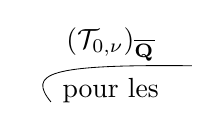
\begin{tikzpicture}[baseline=(words.base)]
\node[anchor=base west,inner sep=0] (words) at (0,0) {pour les};
\node[anchor=base west,inner sep=0] at (0.05,.62) {\inserted{$(\mathcal T_{0,\nu})_{\overline{\mathbf Q}}$}};
\draw[line width=.3pt] (-.14,-.06) .. controls (-.43,.30) and (-.20,.42) .. (1.65,.40);
\end{tikzpicture} courbes de genre $0$ avec $\nu$ points marqués, et famille \deleted{des} modulaire \deleted{\unsure{par}} $\nu$-ponctuée sur $\mathcal T_{0\nu}$\ldots.

Le Topos $(\mathcal T_{0,\nu})_{\mathbf Q}$ pour $\nu=0,1,2$ \uline{n'est} pas un étendu --- car les schémas d'Isom \unsure{d'un|d'une} $X/S$ fibré projectif de rang $1$, avec $\unsure{2|\nu}$ sections marquées (distinctes sur chaque fibre) est lisse de dim rel. $3-\nu\deleted{\unsure{\geq|=|\leq}}>0$ (si $\deleted{\unsure{\nu}}0\leq\nu\leq2$).
\deleted{\unsure{Néanmoins}} \inserted{En fait} ce sont les topos
\figure{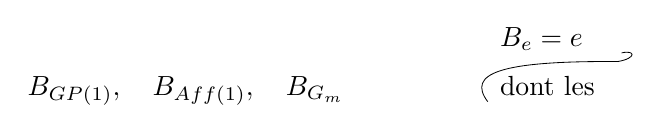
\begin{tikzpicture}[baseline=(list.base)]
\node[anchor=base west,inner sep=0] (list) at (0,0) {$B_{\operatorname{GP}(1)},\quad B_{\operatorname{Aff}(1)},\quad B_{G_m}$};
\node[anchor=base west,inner sep=0] at (6.0,0) {dont les};
\node[anchor=base west,inner sep=0] at (6.0,.62) {$\inserted{B_e=e}$};
\draw[line width=.3pt] (5.85,-.08) .. controls (5.58,.28) and (6.0,.44) .. (7.5,.43) .. controls (7.74,.47) and (7.73,.58) .. (7.55,.54);
\end{tikzpicture}}
\mspage{26}
